\begin{name}
	{\tenchude}
	{TOÁN 12}
	{LỚP TOÁN THẦY PHÁT}
	{Thời gian: 90 phút - Không kể thời gian phát đề}
\end{name}
\Opensolutionfile{ans}[ans/ansDe1-TN1]
\begin{ex}%[2D4N1-1]%[To 20 - Dot 17 - Chuong 4 - Bai 3 - CD - De 1 - TN]%[Nguyễn Hữu Duy]
Nếu hàm số $f(x)$ liên tục trên đoạn $[a;b]$ và $c$ là số thực tùy ý thuộc đoạn $[a;b]$, thì tính chất nào sau đây đúng?
\choice
{\True $\displaystyle\int_a^b f(x) \mathrm{\,d}x = \displaystyle\int_a^c f(x) \mathrm{\,d}x + \displaystyle\int_c^b f(x)\mathrm{\,d}x$}
{$\displaystyle\int_a^b f(x)\mathrm{\,d}x = \displaystyle\int_a^c f(x) \mathrm{\,d}x - \displaystyle\int_c^b f(x) \mathrm{\,d}x$}
{$\displaystyle\int_a^b f(x)\mathrm{\,d}x = \displaystyle\int_a^c f(x)\mathrm{\,d}y + \displaystyle\int_c^b f(x) \mathrm{\,d}z$}
{$\displaystyle\int_a^b f(x)\mathrm{\,d}x = \displaystyle\int_a^c f(x)\mathrm{\,d}y - \displaystyle\int_c^b f(x)\mathrm{\,d}z$}
\loigiai{
Theo định nghĩa tích phân ta có $\displaystyle\int_a^b f(x) \mathrm{\,d}x = \displaystyle\int_a^c f(x) \mathrm{\,d}x + \displaystyle\int_c^b f(x)\mathrm{\,d}x$.
}
\end{ex}

\begin{ex}%[2D4N1-2]
Tìm họ nguyên hàm của hàm số $f(x)=\dfrac{1}{x}+1$. \choice
{$F(x)=-\dfrac{1}{x^2}+x+C$}
{\True $F(x)=\ln |x|+x+C$}
{$F(x)=\ln x+x+C$}
{$F(x)=\ln |x|+C$}
\loigiai{
Họ nguyên hàm của hàm số $f(x)=\dfrac{1}{x}+1$ là $F(x)=\ln |x|+x+C$.}
\end{ex}

\begin{ex}%[2D4H1-3]
Hàm số $F(x)=x\sin x+\cos x+2024$ là một nguyên hàm của hàm số nào trong các hàm số sau?
\choice
{ $f(x)=x\sin x$ }
{ $f(x)=-x\cos x$ }
{ $f(x)=-x\sin x$ }
{\True $f(x)=x\cos x$ }
\loigiai{
$F'(x)=( x\sin x+\cos x+2024 )' = \sin x + x\cos x - \sin x = x\cos x$, $\forall x\in \mathbb{R}$.\\
$\Rightarrow$ Hàm số $F(x)$ là một nguyên hàm của hàm số $f(x)=x\cos x$ trên $\mathbb{R}$.
}
\end{ex}

\begin{ex}%[2D4H2-1]
Cho hàm số $f(x)$ và $F(x)$ liên tục trên $\mathbb{R}$ thoả mãn $F'(x)=f(x)$ với mọi số thực $x$. Tính   $\displaystyle \int\limits_0^1 f(x)\mathrm{\,d}x$. Biết $F(0)=2; F(1)=5$.
\choice
{\True $3$}
{$4$}
{$5$}
{$6$}
\loigiai{
$\displaystyle \int\limits_0^1 f(x)\mathrm{\,d}x = F(1)-F(0)=5-2=3$.
}
\end{ex}

\begin{ex}%[2D4N3-1]
\immini[thm]{Diện tích hình phẳng giới hạn bởi đồ thị hàm số $ y=f(x)$ và trục hoành (phần gạch chéo trong hình vẽ) là
\choice
{\True $ S=\displaystyle\int\limits_{-2}^0f(x)\mathrm{d}x-\displaystyle\int\limits_0^1f(x)\mathrm{d}x$}
{$ S=\displaystyle\int\limits_{-2}^0f(x)\mathrm{d}x+\displaystyle\int\limits_0^1f(x)\mathrm{d}x$}
{$ S=\displaystyle\int\limits_0^1f(x)\mathrm{d}x-\displaystyle\int\limits_{-2}^0f(x)\mathrm{d}x$}
{$\left|\displaystyle\int\limits_{-2}^1f(x)\mathrm{d}x\right|$}
}
{
\begin{tikzpicture}[scale=0.8,>=stealth, font=\footnotesize, line join=round, line cap=round]
\def\a{1} \def\b{-3} \def\c{0} \def\d{2} % Hệ số
\def\xmin{-3} \def\xmax{2}
\def\ymin{-1} \def\ymax{3}
%	\draw[color=gray!50,dashed] (\xmin,\ymin) grid (\xmax,\ymax);
\draw[->] (\xmin,0)--(\xmax,0) node [below]{$x$};
\draw[->] (0,\ymin)--(0,\ymax) node [left]{$y$};
\node at (0,0) [below left]{$O$};
\clip (\xmin+0.1,\ymin+0.1) rectangle (\xmax-0.5,\ymax-0.1);
\draw[smooth,samples=300] plot(\x,{\a*(\x+2)*(\x)*(\x-1)});

\fill[pattern=north east lines,opacity=0.8] plot[domain=-2:1](\x,{\a*(\x+2)*(\x)*(\x-1)})--cycle;
%	\draw[dashed](-1,0)--(-1,-2)
%	(3,0)--(3,2);
\draw[fill=black](-2,0)node[above left]{$-2$}circle(1pt)
(1,0)node[above]{$1$}circle(1pt)
(1.2,1.5)node[above,rotate=80,scale=0.8]{$y=f(x)$}
;
\end{tikzpicture}
}
\loigiai{
Diện tích hình phẳng giới hạn bởi đồ thị hàm số $ y=f(x)$ và trục hoành (phần gạch chéo trong hình vẽ) là $ S=\displaystyle\int\limits_{-2}^1\left| f(x)\right|\mathrm{d}x=\displaystyle\int\limits_{-2}^0f(x)\mathrm{d}x-\displaystyle\int\limits_0^1f(x)\mathrm{d}x$.}
\end{ex}

\begin{ex}%[2D4H3-3]
Tính thể tích vật thể tạo thành khi quay hình phẳng $(H)$ quanh trục $Ox$, biết $(H)$ được giới hạn bởi các đường $y=4x^2-1$, $y=0$.
\choice
{\True $\dfrac{8\pi}{15}$}
{$\dfrac{4\pi}{15}$}
{$\dfrac{16\pi}{15}$}
{$\dfrac{2\pi}{15}$}
\loigiai{
Phương trình hoành độ giao điểm $4x^2-1=0\Leftrightarrow x=\pm\dfrac{1}{2}$.\\
Suy ra $V=\pi\displaystyle\int\limits_{-\frac{1}{2}}^{\frac{1}{2}}(4x^2-1)^2\mathrm{\,d}x=\pi\displaystyle\int\limits_{-\frac{1}{2}}^{\frac{1}{2}}(16x^4-8x^2+1)\mathrm{\,d}x=\pi\left.\left(\dfrac{16}{5}x^5-\dfrac{8}{3}x^3+x\right)\right|_{-\frac{1}{2}}^{\frac{1}{2}}=\dfrac{8\pi}{15}.$
}
\end{ex}

\begin{ex}%[2H5N1-1]
Trong không gian $Oxyz$, phương trình của mặt phẳng $(Oxy)$ là
\choice
{\True $z=0$}
{$x=0$}
{$y=0$}
{$x+y=0$}
\loigiai{
Phương trình của mặt phẳng $(Oxy)$ là $z=0$.
}
\end{ex}

\begin{ex}%[2H5N1-2]
Trong không gian $Oxyz$, cho mặt phẳng $(P)\colon 2x+y-z+3=0$. Véc-tơ nào sau đây là véc-tơ pháp tuyến của mặt phẳng $(P)$?
\choice
{$\overrightarrow{n}_1=(1;-1;3)$}
{$\overrightarrow{n}_2=(2;-1;3)$}
{\True $\overrightarrow{n}_3=(2;1;-1)$}
{ $\overrightarrow{n}_4=(2;1;3)$}
\loigiai{
Mặt phẳng $Ax+By+Cz+D=0$ nhận véc-tơ $\overrightarrow{n}=(A;B;C)$ làm một véc-tơ pháp tuyến.
}
\end{ex}

\begin{ex}%[2H5H1-3]
Cho hai mặt phẳng $(\alpha)\colon  3 x-2 y+2 z+7=0,$ $(\beta)\colon 5 x-4 y+3 z+1=0$. Phương trình mặt phẳng đi qua gốc tọa độ $O$ đồng thời vuông góc với cả $(\alpha)$ và $(\beta)$ là
\choice
{$2 x-y-2 z=0$}
{$2 x-y+2 z=0$}
{\True $2 x+y-2 z=0$}
{$2 x+y-2 z+1=0$}
\loigiai{
Véc-tơ pháp tuyến của hai mặt phẳng lần lượt là $\overrightarrow{n}_\alpha=(3 ;-2 ; 2), \overrightarrow{n}_\beta=(5 ;-4 ; 3)$.\\
Suy ra $\left[\overrightarrow{n}_\alpha ; \overrightarrow{n}_\beta\right]=(2 ; 1 ;-2)$ là véc-tơ pháp tuyến của mặt phẳng cần tìm.\\
Phương trình mặt phẳng đi qua gốc tọa độ $O, $ có véc-tơ pháp tuyến $\vec{n}=(2 ; 1 ;-2)$ là $2 x+y-2 z=0$.
}
\end{ex}

\begin{ex}%[2H5N2-1]%[Dự án 2025 - Đề cấu trúc mới của Bộ theo [Thành Đức Trung]
Trong không gian $Oxyz$, đường thẳng $d\colon \dfrac{x-1}{2}=\dfrac{y-2}{-1}=\dfrac{z-3}{2}$ đi qua điểm nào dưới đây?
\choice
{$M(-1;-2;-3)$}
{\True $P(1;2;3)$}
{$Q(2;-1;2)$}
{$N(-2;1;-2)$}
\loigiai
{
Vì $\dfrac{-1-1}{2}=\dfrac{2-2}{-1}=\dfrac{3-3}{2}=0$ nên đường thẳng $d$ đi qua điểm $P(1;2;3)$.
}
\end{ex}

\begin{ex}%[2H5N2-7]%[Dự án EX-TF-TLN-2024 Đợt 3-  GV. Đỗ Chí Tâm]
Trong không gian $Oxyz$, góc giữa đường thẳng $d:\dfrac{x-3}{2}=\dfrac{y+1}{1}=\dfrac{z-3}{1}$ và mặt phẳng  $(P):x+2y-z+5=0$ là
\choice
{\True $30^{\circ}$}
{ $45^{\circ}$}
{$60^{\circ}$}
{$90^{\circ}$}
\loigiai{
Gọi $\varphi$ là góc giữa $d$ và $(P)$.\\
Đường thẳng $d$ có véc-tơ chỉ phương $\vec{u}=(2;1;1)$, $(P)$ có véc-tơ pháp tuyến $n=(1;2;-1)$.\\
\[\sin \varphi =\dfrac{|\vec{u}\cdot \vec{n}|}{|\vec{u}|\cdot|\vec{n}|}= \dfrac{\left| 2\cdot 1+1\cdot 2+1\cdot (-1)\right|}{\sqrt{2^2+1^2+1^2} \cdot \sqrt{1^2 +2^2+(-1)^2}}=\dfrac{1}{2} \Rightarrow \varphi = 30^{\circ}.\]
}
\end{ex}

\begin{ex}%[2H5H2-4]
Trong không gian $Oxyz$, cho hai đường thẳng $d_{1}  \colon \dfrac{x-3}{-1} =\dfrac{y-3}{-2} =\dfrac{z+2}{1} $; $d_{2}  \colon \dfrac{x-5}{-3} =\dfrac{y+1}{2} =\dfrac{z-2}{1} $ và mặt phẳng $\left(P\right) \colon x+2y+3z-5=0$. Đường thẳng vuông góc với $\left(P\right)$, cắt $d_{1} $ và $d_{2} $ có phương trình là
\choice
{$\dfrac{x-1}{3} =\dfrac{y+1}{2} =\dfrac{z}{1} $}
{$\dfrac{x-2}{1} =\dfrac{y-3}{2} =\dfrac{z-1}{3} $}
{$\dfrac{x-3}{1} =\dfrac{y-3}{2} =\dfrac{z+2}{3} $}
{\True $\dfrac{x-1}{1} =\dfrac{y+1}{2} =\dfrac{z}{3} $}
\loigiai{
Phương trình $d_{1}  \colon \heva{x&=3-t_{1}  \\ y&=3-2t_{1}  \\ z&=-2+t_{1} } $ và $d_{2}  \colon \heva{x&=5-3t_{2}  \\ y&=-1+2t_{2}  \\ z&=2+t_{2}.} $\\
Gọi đường thẳng cần tìm là $\Delta $. \\
Giả sử đường thẳng $\Delta $ cắt đường thẳng $d_{1} $ và $d_{2} $ lần lượt tại $A$, $B$. \\
Gọi $A\left(3-t_{1} ;3-2t_{1} ;-2+t_{1} \right)$, $B\left(5-3t_{2} ;-1+2t_{2} ;2+t_{2} \right)$.\\ $\overrightarrow{AB}=\left(2-3t_{2} +t_{1} ;-4+2t_{2} +2t_{1} ;4+t_{2} -t_{1} \right).$ \\
véc-tơ pháp tuyến của $\left(P\right)$ là $\vec{n}=\left(1;2;3\right)$. \\
Do $\overrightarrow{AB}$ và $\vec{n}$ cùng phương nên $\dfrac{2-3t_{2} +t_{1} }{1} =\dfrac{-4+2t_{2} +2t_{1} }{2} =\dfrac{4+t_{2} -t_{1} }{3} $\\
$\Leftrightarrow \heva{\dfrac{2-3t_{2} +t_{1} }{1} =\dfrac{-4+2t_{2} +2t_{1} }{2}  \\ \dfrac{-4+2t_{2} +2t_{1} }{2} =\dfrac{4+t_{2} -t_{1} }{3} } $$\Leftrightarrow \heva{t_{1} =2. \\ t_{2} =1} $ Do đó $A\left(1;-1;0\right)$, $B\left(2;-1;3\right)$.\\
Phương trình đường thẳng $\Delta $ đi qua $A\left(1;-1;0\right)$ và có véc-tơ chỉ phương $\vec{n}=\left(1;2;3\right)$ là $\dfrac{x-1}{1} =\dfrac{y+1}{2} =\dfrac{z}{3} .$}
\end{ex}
\Closesolutionfile{ans}

\TNTF
\Opensolutionfile{ans}[ans/ansDe1-TN2]
\begin{ex}%[MĐ2]%[2D4H2-4]
Nếu các số hữu tỉ $a,b$ thỏa mãn $\displaystyle\int \limits_0^1(a\mathrm{e}^x+b)\mathrm{d}x=3\mathrm{e}+4$ thì các phát biểu sau đúng hay sai?
\choiceTF[t]
{$a>b$}
{$a=2b$}
{\True $a=3,\, b=7$}
{\True $2a-b=-1$}
\loigiai{
Ta có $\displaystyle\int \limits_0^1(a\mathrm{e}^x+b)\mathrm{d}x=(a\mathrm{e}^x+bx)\bigg|_0^1=a\mathrm{e}+(-a+b)\Rightarrow \heva{&a=3 \\ &-a+b=4} \Rightarrow \heva{&a=3 \\ &b=7.}$\\
\begin{itemchoice}
\itemch Suy ra $a>b$ là sai.
\itemch Do $a=3, \, b=7$ nên $a=2b$ là sai.
\itemch $a=3,\, b=7$ là khẳng định đúng.
\itemch $2a-b= 2\cdot 3-7=-1$ là khẳng định đúng.
\end{itemchoice}
}
\end{ex}

\begin{ex}%[Dat Thai, Dự án Ex-TF-TLN-2024-Dot03]%[2H5H2-5]
Cho đường thẳng $d$ đi qua điểm $A(0; 0; 1)$ có véc-tơ chỉ phương $\overrightarrow{u} = (1; 1; 3)$ và mặt phẳng $(\alpha) \colon 2x + y - z + 5 = 0$.
\choiceTF
{\True $B(2;2;7)\in d$}
{Phương trình đường thẳng $d$ là $\dfrac{x}{1} = \dfrac{y}{1} = \dfrac{z+1}{3}$}
{$\overrightarrow{n} = (2;1;1)$ là một véc-tơ pháp tuyến của mặt phẳng $(\alpha)$}
{\True Đường thẳng $d$ song song với mặt phẳng $(\alpha)$}
\loigiai{
\begin{itemchoice}
\itemch \textbf{Đúng}. Vì $\overrightarrow{AB} = (2;2;6) = 2\overrightarrow{u}$.
\itemch \textbf{Sai}. Vì phương trình đường thẳng $d$ là $\dfrac{x}{1} = \dfrac{y}{1} = \dfrac{z-1}{3}$.
\itemch \textbf{Sai}. Vì họ véc-tơ pháp tuyến của mặt phẳng $(\alpha)$ có dạng $k\cdot(2;1;-1)$ ($k$ khác $0$), nên nếu giả sử $\overrightarrow{n} = (2;1;1)$ là một véc-tơ pháp tuyến của mặt phẳng $(\alpha)$ thì tồn tại số thực $k$ khác $0$ để
\[
\heva{&2 = 2k\\ & 1 = k\\ & 1=-k} \Leftrightarrow\heva{&k=1\\ &k=-1} (\text{vô lí}).
\]
\itemch \textbf{Đúng}. Vì $\vec{n} = (2;1;-1)$ là một véc-tơ pháp tuyến của mặt phẳng $(\alpha)$ thoả mãn
\[
\vec{n} \cdot \vec{u} = 2\cdot 1 + 1\cdot 1 + (-1)\cdot 3 = 0 \text{ hay } \vec{n}\perp \vec{u}
\]
nên $d\parallel (\alpha)$ hoặc $d\subset(\alpha)$.\\
Kết hợp với $A\notin (\alpha)$ ta thu được $d\parallel (\alpha)$.
\end{itemchoice}
}
\end{ex}
\Closesolutionfile{ans}

\TNSA
\Opensolutionfile{ans}[ans/ansDe1-TN3]
\begin{ex}%[2D4H1-1]%[Đào Trung Kiên]
Biết $ F(x) $ là một nguyên hàm của hàm số $ f(x) = \mathrm{e}^{2x} $ và $ F(0) = 0$. Tính giá trị của $F(\ln 3)$.
\shortans[]{$4$}
\loigiai{
Ta có $ \heva{& F(0) = 0 \\ & F(x) = \dfrac{1}{2} \cdot \mathrm{e}^{2x} + C } \Rightarrow F(x) = \dfrac{1}{2} \cdot \mathrm{e}^{2x} - \dfrac{1}{2} \Rightarrow F(\ln 3) =  \dfrac{1}{2}  \cdot \left  (  \mathrm{e}^{ 2 \cdot \ln 3 } - 1 \right ) = 4$.
}
\end{ex}

\begin{ex}%[2D4V3-1]
	\immini{
	Gọi $H$ là hình phẳng giới hạn bởi đồ thị hàm số $y=-x^2+4x$ và trục hoành. Hai đường thẳng $y=m$ và $y=n$ chia $(H)$ thành ba phần có diện tích bằng nhau (tham khảo hình vẽ). Giá trị của biểu thức $T=(4-m)^3+(4-n)^3$ bằng bao nhiêu? (Kết quả làm tròn đến hàng phần mười)
	}{
	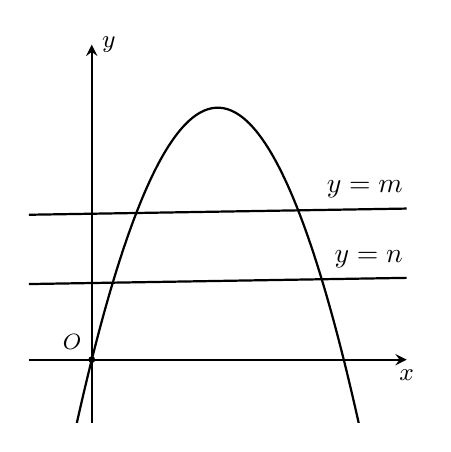
\begin{tikzpicture}[thick,>=stealth,x=1cm,y=1cm,scale=.8]
	\draw[->] (-1,0) -- (5,0) node[below] {\small $x$};
	\draw[->] (0,-1) -- (0,5) node[right] {\small $y$};
	\draw [fill=white,draw=black] (0,0) circle (1pt)node[above left] {\footnotesize $O$};
	\clip(-1,-1) rectangle (5,5);
	\draw[thick,smooth,samples=100,domain=-1:5] plot(\x,{-(\x)^2+4*(\x)});
	\draw (-1,1.2)--(5.1,1.3)node[above left]{$y=n$};
	\draw (-1,2.3)--(5.1,2.4)node[above left]{$y=m$};
	\end{tikzpicture}}
	\shortans[]{$35{,}6$}
	\loigiai{
	\immini{
	Gọi $S$ là diện tích hình phẳng giới hạn bởi đồ thị hàm số $y=-x^2+4x$ và trục $Ox$ và hai đường thẳng $x=0$, $x=2$.\\
	Khi đó $S=\displaystyle\int\limits_{0}^{2} (-x^2+4x)\mathrm{\,d}x =\dfrac{16}{3}$.\\
	Đường thẳng $y=m$ và $y=n$ chia $S$ thành ba phần bằng nhau có diện tích theo thứ tự từ trên xuống là $S_1$; $S_2$; $S_3$.\\
	Gọi hoành độ các giao điểm của parabol với hai đường thẳng như hình bên.\\
	Ta có
	\begin{eqnarray*}
	&& S_1=2\displaystyle\int\limits_{a}^{2} (-x^2+4x-m)\mathrm{\,d}x =\dfrac{1}{3}S\\
	&\Leftrightarrow & \left(-\dfrac{x^3}{3}+2x^2-mx\right)\Big|_{a}^{2}=\dfrac{1}{3}\cdot\dfrac{16}{3}\\
	&\Leftrightarrow & \left(\dfrac{16}{3}-2m\right)-\left(-\dfrac{a^3}{3}+2a^2-ma\right)=\dfrac{16}{9}\quad(1).
	\end{eqnarray*}
	Mà $x=a$ là nghiệm của phương trình $-x^2+4x=m$ nên ta có $-a^2+4a=m\quad(2)$.\\
	Thay $(2)$ vào $(1)$ ta được $-\dfrac{2a^3}{3}+4a^2-8a+\dfrac{32}{9}=0\Leftrightarrow a\approx 0{,}613277$.\\
	Suy ra $m=-a^2+4a\approx 2{,}077$.\\
	Tương tự ta có
	\begin{eqnarray*}
	&& S_1+S_2=\dfrac{2}{3}S\\
	&\Rightarrow & 2\displaystyle\int\limits_{b}^{2} (-x^2+4x-n)\mathrm{\,d}x =\dfrac{2}{3}\cdot 2\cdot\displaystyle\int\limits_{0}^{2} (-x^2+4x)\mathrm{\,d}x\\
	&\Leftrightarrow & -\dfrac{2}{3}b^3+4b^2-8b+\dfrac{16}{9}=0\\
	&\Leftrightarrow & b\approx 0{,}252839\Rightarrow n=-b^2+4b=0{,}947428.
	\end{eqnarray*}
	Khi đó $T=(4-m)^3+(4-n)^3=\dfrac{320}{9}\approx35{,}6$.
	}{
	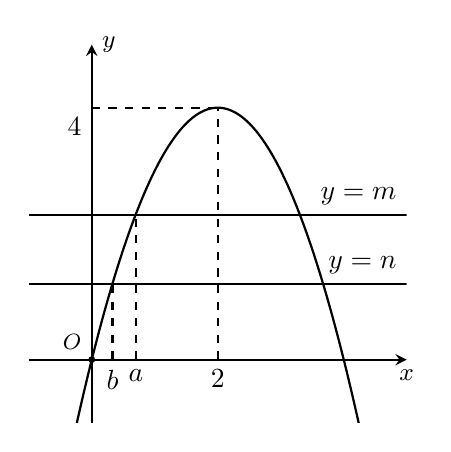
\begin{tikzpicture}[thick,>=stealth,x=1cm,y=1cm,scale=.8]
	\draw[->] (-1,0) -- (5,0) node[below] {\small $x$};
	\draw[->] (0,-1) -- (0,5) node[right] {\small $y$};
	\draw [fill=white,draw=black] (0,0) circle (1pt)node[above left] {\footnotesize $O$};
	\clip(-1,-1) rectangle (5,5);
	\draw[thick,smooth,samples=100,domain=-1:5] plot(\x,{-(\x)^2+4*(\x)});
	\draw (-1,1.2)--(5,1.2)node[above left]{$y=n$};
	\draw (-1,2.3)--(5,2.3)node[above left]{$y=m$};
	\draw[dashed](0.33,0)node[below]{$b$}--(0.33,1.2) (0.7,0)node[below]{$a$}--(0.7,2.3) (2,0)node[below]{$2$}--(2,4);
	\draw[dashed] (0,4) node[below left]{$4$}--(2,4);
	\end{tikzpicture}
	}
	}
	\end{ex}

\begin{ex}%[2H5H2-7]
Gọi $\varphi$ là góc giữa hai đường thẳng $d_1 \colon \dfrac{x-1}{-2}= \dfrac{y+2}{1}= \dfrac{z-3}{2}$ và $d_2 \colon \dfrac{x+3}{1}= \dfrac{y-1}{1}= \dfrac{z+2}{-4}$. Tính $\cos \varphi$ (làm tròn đến hàng phần trăm).
\shortans{$0{,}71$}
\loigiai
{
Đường thẳng $ d_1 $ có một véc-tơ chỉ phương $ \vec u_1 =(-2;1;2)$.\\
Đường thẳng $ d_2 $ có một véc-tơ chỉ phương $ \vec u_2 =(1;1;-4)$.\\
Ta có
\begin{eqnarray*}
\cos \varphi
&=&\left| \cos \left( \vec u_1, \vec u_2 \right)\right| = \dfrac{\left|  \vec u_1 \cdot  \vec u_2 \right|}{\left| { \vec u_1} \right| \cdot \left| { \vec u_2} \right|}\\
&=&\dfrac{|-2 \cdot 1+ 1\cdot 1+ 2\cdot (-4)|}{\sqrt{(-2)^2+1^2+2^2} \cdot \sqrt{1^2+1^2+(-4)^2}}\\
&=& \dfrac{\sqrt {2}}{2} \approx 0{,}71.
\end{eqnarray*}
}
\end{ex}

\begin{ex}%[2H5V1-7]
Một công trình đang xây dựng được gắn hệ trục $Oxyz$ (đơn vị trên mỗi trục tọa độ là mét). Ba bức tường $(P),(Q),(R)$ (như hình vẽ) của tòa nhà lần lượt có phương trình $(P)\colon 2x-y-z+1=0$, $(Q)\colon x+3y-z-2=0,(R)\colon 4x-2y-2z+9=0$. Tính chiều rộng bức tường $(Q)$ của tòa nhà. (Kết quả làm tròn đến hàng phần chục).
\begin{center}
\includegraphics[width=0.7\textwidth]{images/C5B1CD3-H3.png}
\end{center}
\shortans{$2{,}9$}
\loigiai{
\begin{itemize}
\item Kiểm tính song song hoặc vuông góc giữa các bức tường $(P),(Q),(R)$ của tòa nhà.\\
Ta có $(P)$ có vectơ pháp tuyến là $\vec{n}_P=(2;-1;-1)$, $(Q)$ có vectơ pháp tuyến là $\vec{n}_Q=(1; 3;-1)$, $(R)$ có vectơ pháp tuyến là $\vec{n}_R=(4;-2;-2)$.\\
Khi đó $\vec{n}_R=(4;-2;-2)=2(2;-1;-1) \Rightarrow \vec{n}_R=2\vec{n}_P$ nên hai bức tường $(P)$ và $(R)$ song song nhau.\\
Mặt khác $\vec{n}_P \cdot \vec{n}_Q=2\cdot 1+(-1) \cdot 3+(-1) \cdot(-1)=0\Rightarrow \vec{n}_P \perp \vec{n}_Q$ nên bức tường $(Q)$ vuông góc với hai bức tường $(P)$ và $(R)$.
\item Tính chiều rộng bức tường $(Q)$ của tòa nhà.\\
Do hai bức tường $(P)$ và $(R)$ song song nhau nên chiều rộng bức tường $(Q)$ là khoảng cách giữa hai bức tường $(P)$ và $(R)$.\\
Chọn điểm $N(0; 0; 1) \in(P)$. Do hai bức tường $(P)$ và $(R)$ song song nhau nên
\[\mathrm{d}((P),(R))=\mathrm{d}(N,(R))=\dfrac{|4\cdot 0-2\cdot 0-2\cdot 1+9|}{\sqrt{4+1+1}}=\dfrac{7}{\sqrt{6}} \approx 2{,}9.\]
\end{itemize}
}
\end{ex}

\TL
\begin{ex}%[2H5H2-3]%[Dự án 2025 - Đề cấu trúc mới của Bộ theo [Thành Đức Trung]
Trong không gian $Oxyz$, cho tam giác $ABC$ có $A(0;0;1)$, $B(-3;2;0)$, $C(2;-2;3)$. Viết phương trình tham số đường cao kẻ từ $B$ của tam giác $ABC$.
% \shortans{$-2$}
\loigiai
{
Gọi $\Delta$ là đường cao kẻ từ $B$ của tam giác $ABC$.\\
Ta có $\heva{& \overrightarrow{AB}=(-3;2;-1) \\ & \overrightarrow{AC}=(2;-2;2)} \Rightarrow \left[\overrightarrow{AB},\overrightarrow{AC}\right]=(2;4;2)$. \\
Suy ra một véc-tơ pháp tuyến của mặt phẳng $(ABC)$ là $\overrightarrow{n}=(1;2;1)$.\\
Ta có $\heva{ & \Delta \subset(ABC) \\ & \Delta \perp AC}$, suy ra đường thẳng $\Delta$ nhận $\left[\overrightarrow{n},\overrightarrow{AC}\right]$ làm một véc-tơ chỉ phương.\\
Có $\left[\overrightarrow{n},\overrightarrow{AC}\right]=(6;0;-6)=6\overrightarrow{u}$ với $\overrightarrow{u}=(1;0;-1)$. \\
Suy ra đường thẳng $\Delta$ nhận $\overrightarrow{u}=(1;0;-1)$ làm véc-tơ chỉ phương.\\
Do đó phương trình đường thẳng $\Delta$ là $\Delta \colon \heva{ & x=-3+t \\ & y=2 \\ & z=-t}$.
}
\end{ex}

\begin{ex}%[12-MH-2-MH2025]%[MH-2025, Nguyễn Trần Phong]%[2D4C3-2]
	\immini{Chướng ngại vật \lq\lq  tường cong\rq\rq trong một sân thi đấu X-Game là một khối bê tông có chiều cao từ mặt đất lên là $3$ m. Giao của mặt tường cong và mặt đất là đoạn thẳng $AB = 2$ m. Thiết diện của khối tường cong cắt bởi mặt phẳng vuông góc với $AB$ tại $A$ là một hình tam giác vuông cong $ACE$ với $AC = 4$ m, $CE = 3$ m và cạnh cong $AE$ nằm trên một đường Parabol có trục đối xứng vuông góc với mặt đất. Tại vị trí $M$ là trung điểm của $AC$ thì tường cong có độ cao $1$ m. Thể tích bê tông cần sử dụng để tạo nên khối tường cong đó gần nhất với số nào dưới đây?
	\shortans{$9{,}3$}
	}{\begin{tikzpicture}[>=stealth,x=0.8cm,y=0.8cm,scale=0.7]
	\coordinate[label=below:$A$] (A) at (0,0);
	\coordinate[label=left:$B$] (B) at (-2,2);
	\coordinate[label=below:$C$] (C) at (6,0);
	\coordinate[label=right:$E$] (E) at (6,6);
	\coordinate (G) at (2,4);
	\coordinate (H) at (4,1.8);
	\coordinate (D) at ($(C)+(B)-(A)$);
	\coordinate (F) at ($(E)+(D)-(C)$);
	\coordinate[label=below:$M$] (M) at ($(A)!0.5!(C)$);
	\coordinate (K) at ($(A)!0.5!(B)$);
	\coordinate (N) at ($(M)+(0,1.1)$);
	\draw (D)--(C)--(A)--(B) (C)--(E)--(F) (M)--(N);
	\draw[dashed] (B)--(D)--(F);
	\foreach \diem in {A,B,C,D,E,F,M,F}	\fill (\diem)circle(1.5pt);
	%\tkzLabelPoints[above left](D)
	%\tkzLabelSegment[right](M,N){\footnotesize$1$ m}
	%\tkzLabelSegment[left](A,B){\footnotesize$2$ m}
	%\tkzLabelSegment[right](C,E){\footnotesize$3{,}5$ m}
	\draw(-1,.8) node[left]{\footnotesize $2$ m} (3,0.8) node[right]{\footnotesize$1$ m} (6,3) node[right]{\footnotesize$3$ m};
	
	\draw plot[smooth,tension=.65] coordinates{(B) (G) (F)};
	\draw plot[smooth,tension=.65] coordinates{(A) (H) (E)};
	\fill [pattern = north east lines] plot[smooth,tension=.65] coordinates{(A) (H) (E)} (0,0) --(-2,2)--(4,8)--(6,6)--cycle;
	\fill [draw=none, pattern = north east lines, color=white] (0,0) plot[smooth,tension=.65] coordinates{(B) (G) (F)} (-2,2)--(4,2)--cycle;
	\end{tikzpicture}
	}
	\loigiai{
	\immini{Chọn hệ trục tọa độ như hình vẽ.\\
	Gọi $AE \colon y = ax^2 + bx + c$.\\
	Do $AE$ đi qua $A(-4; 0)$ nên ta có $16a - 4b + c = 0$.\\
	Do $E (0; 3)$ thuộc cạnh cong $AE$ nên $c = 3$ (2).\\
	Do $N(-2; 1)$ thuộc cạnh cong $AE$ nên $4a - 2b + c = 1$ (3).\\
	Từ (1), (2), (3) suy ra $a = \dfrac{1}{8}$, $b = \dfrac{5}{4}$, $c = 3 \Rightarrow AE \colon y = \dfrac{1}{8}x^2 + \dfrac{5}{4}x + 3$.\\
	Khi đó $S_{AEC} = \displaystyle\int_{-4}^0\left(\dfrac{1}{8} x^2 + \dfrac{5}{4}x + 3\right) dx = \dfrac{14}{3}\left(m^2\right)$.
	}{\begin{tikzpicture}[>=stealth,x=0.8cm,y=0.8cm,scale=0.7]
	\coordinate[label=below:$A$] (A) at (0,0);
	\coordinate[label=left:$B$] (B) at (-2,2);
	\coordinate[label=below:$C$] (C) at (6,0);
	\coordinate[label=right:$E$] (E) at (6,6);
	\coordinate (G) at (2,4);
	\coordinate (H) at (4,1.8);
	\coordinate[label = above left:$D$] (D) at ($(C)+(B)-(A)$);
	\coordinate[label = above:$F$] (F) at ($(E)+(D)-(C)$);
	\coordinate[label=below:$M$] (M) at ($(A)!0.5!(C)$);
	\coordinate (K) at ($(A)!0.5!(B)$);
	\coordinate[label=above left:$N$] (N) at ($(M)+(0,1.1)$);
	\draw (D)--(C)--(A)--(B) (C)--(E)--(F) (M)--(N);
	\draw[dashed] (B)--(D) (D)--(F);
	\foreach \diem in {A,B,C,D,E,F,M,F,N}	\fill (\diem)circle(1.5pt);
	\coordinate (x) at ($(M)!1.5!(C)$);
	\draw[->](C)--(x); \draw (x) node[right]{$x$};
	\coordinate (y) at ($(C)!1.4!(E)$);
	\draw[->](E)--(y); \draw (y) node[right]{$y$};
	%\tkzLabelPoints[above left](D)
	%\tkzLabelSegment[right](M,N){\footnotesize$1$ m}
	%\tkzLabelSegment[left](A,B){\footnotesize$2$ m}
	%\tkzLabelSegment[right](C,E){\footnotesize$3{,}5$ m}
	\draw plot[smooth,tension=.65] coordinates{(B) (G) (F)};
	\draw plot[smooth,tension=.65] coordinates{(A) (H) (E)};
	\fill [pattern = north east lines] plot[smooth,tension=.65] coordinates{(A) (H) (E)} (0,0) --(-2,2)--(4,8)--(6,6)--cycle;
	\fill [draw=none, pattern = north east lines, color=white] (0,0) plot[smooth,tension=.65] coordinates{(B) (G) (F)} (-2,2)--(4,2)--cycle;
	\end{tikzpicture}
	}
	\noindent Thể tích khối tường cong là $V = S_{AEC} \cdot AB = \frac{14}{3} \cdot 2 = \dfrac{28}{3} = 9{,}3\left(\mathrm{~m}^3\right)$.	}
	\end{ex}

\begin{ex}%[2H5C1-7]
Người ta thiết kế một mái che hình chữ nhật $ ABCD $ phía trên sân khấu. Gắn hệ trục tọa độ $ Oxyz $ (đơn vị trên trục là mét), người ta xác định được toạ dộ của các điểm như sau: $ A(0;0;8)$, $B(0;20;8)$, $D(15;0;14)$, $C(15;20;14) $. Một cổng chào hình chữ nhật $ EFHG $ với tọa độ điểm $ G(8;0;4) $ dựng vuông góc với mặt đất. Người ta muốn làm các đoạn dây nối thanh ngang $ GE $ với mái che để gắn hoa và đèn led. Độ dài ngắn nhất của mỗi đoạn dây này bằng bao nhiêu mét? (làm tròn đến chữ số thập phân thứ nhất)
\begin{center}
\includegraphics[scale=.3]{images/2P5-1-H5-16}
\end{center}
\shortans{$1{,}8$}
\loigiai{
Ta có $ A(0;0;8)$, $B(0;20;8)$, $D(15;0;14)$, $C(15;20;14) $.\\
Ta có $ \vec{AB}=(0;20;0) $, $\vec{AC}=(15;20;6)$ nên $ \vec{n}_1=\left[\vec{AB},\vec{AC}\right]=(80;0;300) $ là vectơ pháp tuyến của $ (ABCD) $.\\
Mà mặt phẳng mái che $ (ABCD) $ qua $ A(0;0;8)$ nên có phương trình
\[ 80(x-0)+0(y-0)+300(z-8)=0\Leftrightarrow 4x+15z-120=0 .\]
Độ dài ngắn nhất của dây nối thanh ngang $ GE $ với mái che là khoảng cách từ $ G $ đến mái che (mặt phẳng $ ABCD $) là \[ \mathrm{d}(G,(ABCD))=\dfrac{|4\cdot8+0+15\cdot4-120|}{\sqrt{4^2+0^2+15^2}}=\dfrac{28}{\sqrt{241}}=1{,}8\ (\text{m}). \]
}
\end{ex}
\Closesolutionfile{ans}


% \Closesolutionfile{ansbook}
% \HetDe
% \label{De1}
% %
% \cleardoublepage
% \setcounter{page}{1}
% \rfoot{Trang \thepage/\pageref{DA1} - Đáp án trắc nghiệm Mã đề 1}
% \begin{center}
% 	\bfseries ĐÁP ÁN TRẮC NGHIỆM MÃ ĐỀ 1
% \end{center}

% \inputansbox{10}{ans/ansDe1-TN1}
% \inputansbox[3]{2}{ans/ansDe1-TN2}
% \inputansbox{3}{ans/ansDe1-TN3}
% \label{DA1}
% %
